%%%%%%%%%%%%%%%%%%%%%%%%%%%%%%%%%%%%%%%%%%%%%%%%%%%%%%%%%%%%%%%%%%%%%%%%%%%%%%%%%%%%%%%%%%%%%%%%%%%
%%%%%%%%%%%%%%%%%%%%%%%%%%%%%%%%%%%%%%%%%%%%%%%%%%%%%%%%%%%%%%%%%%%%%%%%%%%%%%%%%%%%%%%%%%%%%%%%%%%
\chapter{Parte fisiol\'ogica}

Esta parte tiene partes copiadas del protocolo de G\'enesis: es temporal. Tiene mucho sentido
que, como la tesis tiene enfoque matem\'atico, deba citar el trabajo de personas enfocadas al
\'area de fisiolog\'ia. Dentro de poco escribir\'e mi propia revisi\'on, aunque sea de la misma
bibliograf\'ia.

\section{Adulto mayor}

Un adulto mayor, de acuerdo a la Organización Mundial de la Salud [2,4], son aquellas personas de 60 a 74 años y son considerados de edad avanzada, de 75 a 90 viejas o ancianas, y las que sobrepasan los 90 se les denomina grandes viejos o longevos. A todo individuo mayor de 60 años se le llamará indistintamente persona de la tercera edad. Un adulto mayor es un individuo que tenga de edad 60 años o más que viva en países en vías de desarrollo y de 65 años o más en los que viven en países desarrollados (3) 

\subsection{ Envejecimiento}
	El envejecimiento es un proceso biológico que se caracteriza por la disminución de las funciones que hacen más susceptible al ser humano de padecer enfermedades y morir a consecuencia de ellas [1]. Durante esta etapa ocurren cambios biológicos, psicológicos y sociales, normales e inherentes a todo individuo debido a que el organismo va perdiendo la habilidad para responder ante el estrés y mantener la regulación homeostática y metabólica, teniendo como consecuencia la disminución de las capacidades cognitivas y de sobrevivencia, reflejándose en la imposibilidad de adaptarse a situaciones de restricción o sobrecarga de cualquier tipo [4,9,10]
	A pesar de ser un proceso natural, no todos los individuos envejecen de la misma forma debido a que la calidad de vida y funcionalidad durante la vejez está relacionada con los aprendizajes adquiridos durante la infancia, adolescencia y edad adulta [11]. Los estilos de vida, los factores de riesgo, la accesibilidad a la educación y la promoción de la salud adoptados a lo largo de la vida son fundamentales al momento de llegar a esta etapa para que en el presente de esta se logre autonomía, a pesar de la edad y los padecimientos que se tengan [1].
	En lo que concierne al ser humano se reconocen tipos diferentes de envejecimiento, entre los que sobresalen el individual y el demográfico o poblacional. El envejecimiento individual es el proceso de evolución que experimenta cada persona en el transcurso de su vida mientras que el envejecimiento poblacional es el incremento del número de adultos mayores con respecto al conjunto de la población a que pertenecen. Esta dualidad de interpretaciones hace que el análisis del envejecimiento deba hacerse en 2 planos diferentes: el social (con implicaciones y dimensiones del micromundo y macromundo) y el individual[12].
	En este sentido, factores como el descenso de la mortalidad general, el aumento de la esperanza de vida y la reducción de la natalidad, dan lugar a un proceso conocido como envejecimiento poblacional, es decir, un proceso que implica una creciente participación de los adultos mayores en la estructura poblacional. Sin embargo, la población de jóvenes y adultos en edad productiva atraviesa por una etapa de crecimiento heredada de periodos de alta fecundidad del pasado.


\section{Morfolog\'a neuronal y cambios en la anatomía cerebral con la vejez (fisiolog\'ia)}

El envejecimiento considerado normal viene determinado por una serie de procesos moleculares, 
celulares, fisiol\'ogicos y psicol\'ogicos que conducen directamente al deterioro de funciones 
cognitivas, específicamente en la atenci\'on y memoria \cite{Navarrete03,Park09}.

En un principio se consideraba que el envejecimiento cerebral ocurr\'ia fundamentalmente por una 
muerte neuronal programada \cite{Coleman87}, sin embargo, estudios realizados con tejido cerebral 
post mortem de adultos mayores que en vida fueron sanos, mostraron que dicha muerte neuronal no 
alcanza un 10\% en su totalidad \cite{Esiri07}. En este sentido, los cambios morfol\'gicos que 
sufren las neuronas durante el envejecimiento son abundantes, observ\'andose una importante 
disminuci\'on de la arborizaci\'n dendr\'itica as\'i como en la densidad y volumen \cite{Hita14}. 
La disminución en la arborización dendr\'itica y de las espinas dendr\'iticas de las neuronas 
piramidales de la corteza prefrontal, temporal superior, pre central y occipital \cite{Hita14}. 
Dichas alteraciones morfol\'ogicas conducen durante el envejecimiento a una disminuci\'on de 
la densidad sin\'aptica y a una desmielinizaci\'on ax\'onica en neuronas de la 
neocorteza \cite{Terry}.

Con el paso del tiempo, la organizaci\'on an\'atomo-funcional del cerebro sufre modificaciones 
que traen como consecuencia la afectaci\'on de diferentes capacidades cognitivas, sin embargo, 
la vulnerabilidad de los circuitos neuronales ante los procesos que ocurren durante el 
envejecimiento no suceden de forma homogénea en todo el cerebro \cite{Hita14}.

Por otro lado, la relevancia del estudio de los cambios anat\'omicos asociados al envejecimiento 
fisiol\'ogico ha ido aumentando al permitir evaluar como dichos cambios se correlacionan con 
el deterioro funcional y cognitivo que caracteriza a las personas mayores, facilita la 
identificaci\'on de estadios tempranos de diferentes patolog\'ias neurodegenerativas estableciendo 
diferencias entre estas y los cambios asociados al envejecimiento fisiol\'ogico \cite{Hita14}.

Durante el envejecimiento, el cerebro sufre una afectaci\'n progresiva del peso \cite{Dekaban78} 
y volumen \cite{Hubbard81} cambios atribuidos a la reducci\'on de sustancia gris y blanca en
las regiones c\'ortico-subcorticales \cite{Hita14}.

Consecuencia de la disminuci\'on de la sustancia gris cortical, se produce una reducci\'on de 
la girificaci\'on en las circunvoluciones, as\'i como un incremento de la profundidad y 
expansi\'on de los surcos de la corteza, siendo estos fen\'omenos ms acentuados en los l\'obulos 
frontales, temporales y parentales, y mucho menos evidentes en la corteza occipital \cite{Raz05}.

Los cambios de presi\'on externa producidos por la dilataci\'on de las astas frontales y por la 
disminuci\'on de la sustancia blanca peri ventricular durante la etapa del envejecimiento 
provocan tambi\'en un aumento del espacio ventricular que conduce a la expansi\'on del l\'iquido 
cerebroespinal \cite{Hita14,Raz05}.
Durante el envejecimiento se reduce significativamente el volumen de estructuras subcorticales 
como la am\'igdala \cite{Allen05}, el n\'ucleo caudado \cite{Raz05}, el t\'alamo 
\cite{CarrilloMora} y el cerebelo \cite{Hita14}.

%%%%%%%%%%%%%%%%%%%%%%%%%%%%%%%%%%%%%%%%%%%%%%%%%%%%%%%%%%%%%%%%%%%%%%%%%%%%%%%%%%%%%%%%%%%%%%%%%%%

\section{El sue\~no}

(Esta secci\'on tambi\'en es copiada, por el momento)

El sue\~no se define como un proceso vital c\'iclico complejo y activo, compuesto por varias 
fases y que posee una estructura interna caracter\'istica, con diversas interrelaciones en los 
sistemas hormonales y nerviosos \cite{FernandezConde07}. Una suspensi\'on f\'acilmente reversible 
de la interacci\'on sensoriomotriz con el medio ambiente, por lo general asociados con el 
dec\'ubito y la inmovilidad.

El sue\~no se determina por cuatro dimensiones diferentes: tiempo circadiano (esto es la hora 
del d\'ia en que se localiza); factores intr\'insecos del organismo (edad, sexo, patrones de 
sue\~o, estado fisiol\'ogico o necesidad de dormir, entre otros); conductas que facilitan o 
inhiben el sue\~no; y el ambiente. Las dos \'ultimas dimensiones se relacionan con la higiene 
del sueño, que incluye las pr\'acticas necesarias para mantener un sue\~no nocturno y una 
vigilancia diurna normales \cite{Sierra02}.

Las caracter\'isticas conductuales que se asocian con el sue\~no en el ser humano pueden 
enumerarse de la siguiente forma\cite{CarrilloMora} 
\begin{enumerate}
\item Disminuci\'on de la conciencia y reactividad a los est\'imulos externos
\item Se trata de proceso f\'acilmente reversibles (lo cual lo diferencia de otros estados 
patol\'ogicos como el estupor y el coma)
\item Se asocia a inmovilidad y relajaci\'on muscular
\item Suele presentarse con una periodicidad circadiana (diaria)
\item Durante el sue\~no los individuos adquieren una postura estereotipada
\item La ausencia de sue\~no (privaci\'on), induce distintas alteraciones conductuales y 
fisiol\'ogicas, adem\'as de que genera una ''deuda'' acumulativa de sueño que eventualmente 
deber\'a recuperarse 
\end{enumerate}

%%%%%%%%%%%%%%%%%%%%%%%%%%%%%%%%%%%%%%%%%%%%%%%%%%%%%%%%%%%%%%%%%%%%%%%%%%%%%%%%%%%%%%%%%%%%%%%%%%%

\subsection{Fisiolog\'ia del sueño}

Los organismos vivos tienen su propio ritmo de actividad y reposo, mismos que desencadenan en la 
percepci\'on de ciclos naturales tales como la sucesión del d\'ia y la noche. En este sentido, 
el sustrato neurol\'ogico relacionado con la ritmicidad del sueño se encuentra en el hipot\'alamo, 
estructura que tiene diversidad de conexiones en el Sistema Nervioso Central, con el fin de 
ejercer una funci\'on o funciones capaces de sincronizar el organismo 
\cite{FernandezConde07,Cabrera14}.

Diversos y muy importantes procesos fisiol\'ogicos y cerebrales, est\'an estrechamente 
relacionados o determinados por el sue\~no o la periodicidad del mismo. A este respecto, existen 
diversas teor\'ias acerca de las funciones del sue\~no, por ejemplo: 
\begin{enumerate}
\item Restablecimiento o conservaci\'on de la energ\'ia
\item Eliminaci\'on de radicales libres acumulados durante el d\'ia
\item Regulaci\'on y restauraci\'on de la actividad el\'ectrica cortical
\item Regulación t\'ermica
\item Regulación metabólica y endocrina
\item Homeostasis sin\'aptica
\item Activaci\'on inmunol\'ogica
\item Consolidaci\'on de la memoria
\end{enumerate}

Las estructuras l\'imbicas, tales como la am\'igdala y el hipot\'alamo, tambi\'en estar\'ian 
activadas, lo que explicar\'ia los fen\'omenos emotivos durante la fase de sue\~no REM ya que 
las emociones est\'an directamente vinculadas con estas zonas cerebrales \cite{Bonet08}.

%%%%%%%%%%%%%%%%%%%%%%%%%%%%%%%%%%%%%%%%%%%%%%%%%%%%%%%%%%%%%%%%%%%%%%%%%%%%%%%%%%%%%%%%%%%%%%%%%%%

\subsection{Funci\'on del sue\~no}

Los efectos del sue\~no no se limitan al propio organismo (necesidad de restauración neurol\'ogica
y la salud), sino que influyen en el desarrollo y funcionamiento normal de un individuo en la 
sociedad, afectando el rendimiento laboral o escolar \cite{Sierra02,Baez05,Rosales06,Marin08}, 
el bienestar psicosocial \cite{BuelaCasal04,Vassali09,Gibson06}, la seguridad vial, entre 
otras \cite{Fontana14}.

Dentro de los factores que se pueden ver afectados por la disminuci\'on de las horas de sue\~no 
se encuentra la calidad del sue\~no, la cual no s\'olo se refiere al hecho de dormir bien durante 
la noche, sino que incluye también un buen funcionamiento diurno. 

%%%%%%%%%%%%%%%%%%%%%%%%%%%%%%%%%%%%%%%%%%%%%%%%%%%%%%%%%%%%%%%%%%%%%%%%%%%%%%%%%%%%%%%%%%%%%%%%%%%
%%%%%%%%%%%%%%%%%%%%%%%%%%%%%%%%%%%%%%%%%%%%%%%%%%%%%%%%%%%%%%%%%%%%%%%%%%%%%%%%%%%%%%%%%%%%%%%%%%%

\section{Etapas del sue\~no}

El sueño normal se divide en dos etapas: sueño REM (Rapid-eyemovement) o también conocido como sueño MOR (movimiento-ocular-rápido) y sueño no-REM, los cuales se diferencian fundamentalmente por sus rasgos electroencefalográficos y una serie de características fisiológicas 51
Una herramienta tecnológica que ha sido de vital importancia para el estudio de la fisiología del sueño es el electroencefalograma (EEG). De forma muy simplificada, el EEG es el la representación gráfica y digital de las oscilaciones que muestra la actividad eléctrica del cerebro, al ser registrada mediante electrodos colocados encima de la piel cabelluda en distintas regiones de la cabeza 4
El sueño MOR se caracteriza por la presencia de ondas de bajo voltaje y alta frecuencia en el electroencefalograma, atonía muscular y movimientos oculares rápidos, además es donde se presentan la mayoría de los sueños. El sueño no- MOR se compone de cuatro fases, 1 y 2, que son de sueño ligero, y 3 y 4 de sueño profundo, las mismas que transcurren de manera secuencial desde la primera hasta la cuarta fase, que es la fase reparadora del sueño, aquella que produce en la persona la sensación de haber descansado cuando se levanta 13,22,43.
Las características de las fases del sueño no-MOR incluyen cuatro etapas, la primera que corresponde a la transición de la vigilia al sueño; la etapa 2 es la intermedia (mayor porcentaje del tiempo de sueño) y en el EEG aparecen husos de sueño y los complejos K. La etapa 3 es la del sueño relativamente profundo, representado en el electroencefalograma por ondas lentas de gran amplitud, y la etapa 4o de sueño profundo con más del 50\% de ondas lentas de gran amplitud13.
	Durante el estado de alerta, mientras se mantienen los ojos cerrados, en el EEG se observan oscilaciones de la actividad eléctrica que suelen encontrarse entre 8-13 ciclos por segundo (Hz), principalmente a nivel de las regiones occipitales (ritmo alfa). Durante el sueño ocurren cambios característicos de la actividad eléctrica cerebral que son la base para dividir el sueño en varias fases. Como ya se mencionó, el sueño suele dividirse en dos grandes fases que, de forma normal, ocurren siempre en la misma sucesión: todo episodio de sueño comienza con el llamado sueño sin movimientos oculares rápidos (No MOR), que tiene varias fases, y después pasa al sueño con movimientos oculares rápidos (MOR). La nomenclatura acerca de las fases del sueño ha sido recientemente modificada por la Academia Americana de Medicina del Sueño (2007)52. Quedó de la siguiente manera:

%%%%%%%%%%%%%%%%%%%%%%%%%%%%%%%%%%%%%%%%%%%%%%%%%%%%%%%%%%%%%%%%%%%%%%%%%%%%%%%%%%%%%%%%%%%%%%%%%%%

\subsection{Sueño No MOR}

Fase 1 (ahora denominada N1): esta fase corresponde con la somnolencia o el inicio del sueño ligero, en ella es muy fácil despertarse, la actividad muscular disminuye paulatinamente y pueden observarse algunas breves sacudidas musculares súbitas que a veces coinciden con una sensación de caída (mioclonías hípnicas), en el EEG se observa actividad de frecuencias mezcladas, pero de bajo voltaje y algunas ondas agudas (ondas agudas del vértex). Fase 2 (ahora denominada N2): en el EEG se caracteriza por que aparecen patrones específicos de actividad cerebral llamados husos de sueño y complejos K; físicamente la temperatura, la frecuencia cardiaca y respiratoria comienzan a disminuir paulatinamente. Fases 3 y 4 o sueño de ondas lentas (en conjunto llamadas fase N3): esta es la fase de sueño No MOR más profunda, y en el EEG se observa actividad de frecuencia muy lenta (< 2 Hz)53.

%%%%%%%%%%%%%%%%%%%%%%%%%%%%%%%%%%%%%%%%%%%%%%%%%%%%%%%%%%%%%%%%%%%%%%%%%%%%%%%%%%%%%%%%%%%%%%%%%%%

\subsection{Sueño MOR}

Ahora es llamado fase R y se caracteriza por la presencia de movimientos oculares rápidos; físicamente el tono de todos los músculos disminuye (con excepción de los músculos respiratorios y los esfínteres vesical y anal), así mismo la frecuencia cardiaca y respiratoria se vuelve irregular e incluso puede incrementarse y existe erección espontánea del pene o del clítoris. Durante el sueño MOR se producen la mayoría de las ensoñaciones (lo que conocemos coloquialmente como sueños), y la mayoría de los pacientes que despiertan durante esta fase suelen recordar vívidamente el contenido de sus ensoñaciones53.
Por otro lado, las necesidades de sueño son muy variables según la edad y las circunstancias individuales 43,54:
Un niño recién nacido duerme casi todo el día, con una proporción próxima al 50\% del denominado sueño «activo», que es el equivalente del sueño MOR. A lo largo de la lactancia los períodos de vigilia son progresivamente más prolongados y se consolida el sueño de la noche; además, la proporción de sueño MOR desciende al 25-30 \%, que se mantendrá durante toda la vida. Entre el 1er y 3er año de vida el niño ya sólo duerme una o dos siestas. Entre los 4 y 5 años y la adolescencia los niños son hipervigilantes, muy pocos duermen siesta, pero tienen un sueño nocturno de 9-10 horas bien estructurado en 5 ciclos o más. Por lo que se refiere a los individuos jóvenes, en ellos reaparece en muchos casos la necesidad fisiológica de una siesta a mitad del día43,55.
La necesidad de sueño en un adulto puede oscilar entre 5 y 9 horas. Asimismo, varía notablemente el horario de sueño entre noctámbulos y madrugadores. En épocas de mucha actividad intelectual o de crecimiento o durante los meses del embarazo, puede aumentar la necesidad de sueño, mientras que el estrés, la ansiedad o el ejercicio físico practicado por la tarde pueden reducir la cantidad de sueño. Los estudios efectuados en individuos aislados de influencias exteriores han mostrado que la tendencia fisiológica general es a retrasar ligeramente la fase de sueño con respecto al ciclo convencional de 24 horas y a dormir una corta siesta “de mediodía” 43,56. Un adulto joven pasa aproximadamente entre 70-100 min en el sueño no MOR para después entrar al sueño MOR, el cual puede durar entre 5-30 min, y este ciclo se repite cada hora y media durante toda la noche de sueño. Por lo tanto, a lo largo de la noche pueden presentarse normalmente entre 4 y 6 ciclos de sueño MOR 22
Por otro lado, en los ancianos se va fragmentando el sueño nocturno con frecuentes episodios de despertar y se reduce mucho el porcentaje de sueño en fase IV y no tanto el de sueño MOR, que se mantiene más constante a lo largo de la vida. Las personas de edad avanzada tienen tendencia a aumentar el tiempo de permanencia en la cama. Muchas de ellas dormitan fácilmente durante el día varias siestas cortas43.

%%%%%%%%%%%%%%%%%%%%%%%%%%%%%%%%%%%%%%%%%%%%%%%%%%%%%%%%%%%%%%%%%%%%%%%%%%%%%%%%%%%%%%%%%%%%%%%%%%%

\subsection{Alteraciones del ciclo vigilia-sueño}

La relevancia que tiene el sueño para para la supervivencia de un individuo es la cantidad de horas que este duerme a lo largo de su vida, mismas que depende fundamentalmente de sus necesidades fisiológicas y de las demandas del ambiente al que está expuesto 4,57
 En el caso de los humanos, es posible establecer una clasificación de patrones de sueño en función de su duración (corta, intermedia y larga) 4. Las personas que muestran un patrón de sueño intermedio, es decir, duración aproximada de entre 7-8 horas, presentan un mejor estado de salud a lo largo de su vida, comparado con los individuos de duración de sueño corta o excesivamente larga que frecuentemente tienen de problemas de salud y/o laborales 42,45,46 . 
La estabilidad del sueño nocturno es otro factor a tener en cuenta debido a que es razonable pensar que un sueño muy fragmentado no cumplirá con sus funciones fisiológicas de igual forma que un patrón de sueño estable a lo largo de la noche. Al respecto, los adultos mayores informan que duermen menos durante la noche, y se acuestan y se despiertan más temprano de lo habitual. Además, tardan más tiempo en conciliar el sueño, se despiertan con más frecuencia durante la noche y la duración de estos despertares es más prolongada 58,59.
La disminución del tiempo de sueño asociada a un incremento de la somnolencia diurna incide negativamente en la función cerebral del día siguiente 60
Por otro lado, existen diversas formas de pérdida de sueño13,25,46: a) la privación de sueño, que quiere decir la suspensión total del sueño por un periodo ($>$ 24 h), b) la restricción del sueño, que significa una disminución del tiempo habitual de sueño, generalmente de forma crónica, y c) la fragmentación del sueño, que significa la interrupción repetida (despertares) de la continuidad del sueño14. Todos estos tipos de alteraciones del sueño han demostrado afectar distintas funciones cognitivas y variedades de memoria en mayor o menor grado.
Las alteraciones de sueño específicamente en personas mayores se han asociado con la presencia de enfermedades crónicas, problemas físicos y de salud mental 3

%%%%%%%%%%%%%%%%%%%%%%%%%%%%%%%%%%%%%%%%%%%%%%%%%%%%%%%%%%%%%%%%%%%%%%%%%%%%%%%%%%%%%%%%%%%%%%%%%%%
%%%%%%%%%%%%%%%%%%%%%%%%%%%%%%%%%%%%%%%%%%%%%%%%%%%%%%%%%%%%%%%%%%%%%%%%%%%%%%%%%%%%%%%%%%%%%%%%%%%

\section{El electroencefalograma}

[Esta parte esta copiada y pegada de ''The origin of biopotentials'' de John William Clark \cite{clark98},
bajo las mismas consideraciones que el marco teorico del protocolo de investigacion de genesis:
deberia ser capaz de escribir mi propio resumen, y solo es cuestion del tiempo que tardare en escribirlo
PERO por lo mientras pondre esto aqui]

The background electrical activity of the brain in unanesthetized animals was
described qualitatively in the nineteenth century, but it was first analyzed in a
systematic manner by the German psychiatrist Hans Berger, who introduced
the term electroencephalogram (EEG) to denote the potential fluctuations
recorded from the brain. Conventionally, the electrical activity of the brain is
recorded with three types of electrodes—scalp, cortical, and depth electro-
des. When electrodes are placed on the exposed surface (cortex) of the brain,
the recording is called an electrocorticogram (ECoG). Thin insulated needle
electrodes of various designs may also be advanced into the neural tissue of
the brain, in which case the recording is referred to as a depth recording.
(There is surprisingly little damage to the brain tissue when electrodes of
appropriate size are employed.) Whether obtained from the scalp, cortex, or
depths of the brain, the recorded fluctuating potentials represent a superpo-
sition of the field potentials produced by a variety of active neuronal current
generators within the volume-conductor medium. Unlike the relatively
simple bioelectric source considered in Section 4.2 (the nerve trunk with
its enclosed bundles of circular cylindrical nerve axons), the sources gener-
ating these field potentials are aggregates of neuronal elements with complex
interconnections. The neuronal elements mentioned previously are the
dendrites, cell bodies (somata), and axons of nerve cells. Moreover, the
architecture of the neuronal brain tissue is not uniform from one location to
another in the brain. Therefore, prior to undertaking any detailed study of
electroencephalography, we first discuss necessary background information
regarding (1) the gross anatomy and function of the brain, (2) the ultra-
structure of the cerebral cortex, (3) the field potentials of single neurons
leading to an interpretation of extracellular potentials recorded in the
cerebral cortex, and (4) typical clinical EEG waveforms recorded via scalp
electrodes. We shall then focus on the general volume-conductor problem in
electroencephalography and briefly discuss abnormal EEG waveforms
(Sherman and Walterspacher, 2006).

%%%%%%%%%%%%%%%%%%%%%%%%%%%%%%%%%%%%%%%%%%%%%%%%%%%%%%%%%%%%%%%%%%%%%%%%%%%%%%%%%%%%%%%%%%%%%%%%%%%

%\subsection{INTRODUCTION TO THE ANATOMY AND FUNCTION OF THE BRAIN}
%
%The central nervous system (CNS) consists of the spinal cord lying within the
%bony vertebral column and its continuation, the brain, lying within the skull
%[Figure 4.24]. The brain is the greatly modified and enlarged portion of the
%CNS, surrounded by three protective membranes (the meninges) and enclosed
%within the cranial cavity of the skull. The spinal cord is likewise surrounded by
%downward continuations of the meninges, and it is encased within the protec-
%tive bony vertebral column. Both brain and spinal cord are bathed in a special
%extracellular fluid called cerebral spinal fluid (CSF).
%Division of the brain into three main parts—cerebrum, brainstem, and
%cerebellum—provides a useful basis for the study of brain localization and
%function (Figure 4.24). The brainstem (medulla, pons, midbrain, diencephalon)
%is the oldest part of the brain. It is actually a short extension of the spinal cord and
%
%\begin{figure}
%\centering
%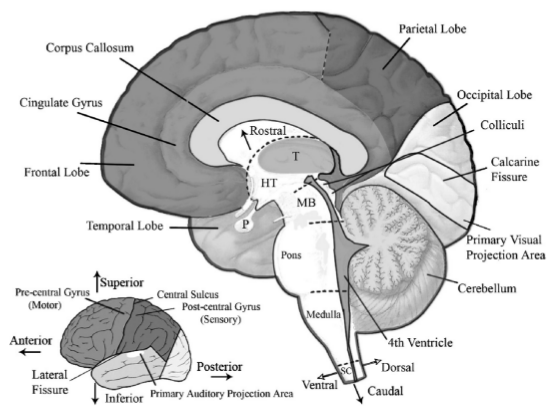
\includegraphics[width=0.7\linewidth]{figura_1.png} 
%\caption{Anatomical relationship of brainstem structures [medulla oblon-
%gata, pons, midbrain, and diencephalon (thalamus and hypothalamus)] to the
%cerebrum and cerebellum. General anatomic directions of orientation in the
%nervous system are superimposed on the diagrams. Here the terms rostral
%(toward head), caudal (toward tail), dorsal (back), and ventral (front) are
%associated with the brainstem; remaining terms are associated with the cerebrum.
%The terms medial and lateral imply nearness and remoteness, respectively, to or
%from the central midline axis of the brain. Symbols: T (thalamus), HT (hypo-
%thalamus), MB (midbrain), SC (spinal cord), P pituitary gland). (Adapted from
%John H. Martin, Neuroanatomy: Text and Atlas, 2nd ed., 1996, pp 14–15, with
%permission of Appleton and Lange, a Simon and Schuster Company.)}
%\end{figure}
%
%serves three major functions: (1) a connecting link between the cerebral cortex,
%spinal cord, and cerebellum; (2) an integrative center for several visceral
%functions (e.g., control of blood pressure and ventilation); and (3) an integration
%center for various motor reflexes. The diencephalon is the most superior portion
%of the brainstem; its chief component and largest structure is the thalamus. The
%thalamus serves as a major relay station and integration center for all of the
%general and special sensory systems, sending information to their respective
%cortical reception areas. It serves as the gateway to the cerebrum. Another major
%component of the diencephalon is the hypothalamus, which integrates functions
%of the autonomic nervous system and along with the pituitary gland, regulates
%functions of the thyroid, adrenal, and reproductive glands. The cerebellum is a
%coordinator in the voluntary (somatic) muscle system and acts in conjunction
%with the brainstem and cerebral cortex to maintain balance and provide harmo-
%nious muscle movements. The larger cerebrum occupies a special dominant
%position in the central nervous system, and conscious functions of the nervous
%system are localized within this structure.
%Within the CNS there are ascending (sensory) nerve tracts that run from
%the spinal cord or brain stem to various areas of the brain, conveying
%information regarding changes in the external environment of the body that
%are reported by various peripheral biological sensors. There are a variety of
%such sensors, including the general sensors of temperature, pain, fine touch,
%pressure, as well as the special senses of vision, audition, equilibrium, taste, and
%olfaction. Figure 4.25 shows the basic plan associated with the general sense
%pathways from the periphery (e.g., skin, muscles) to the cortex. A three-neuron
%chain is involved in conveying information to the cortex where the primary
%neuron has its cell body in a ganglion outside the CNS and makes synaptic
%contact with a secondary neuron whose cell body is located in a nucleus within
%
%\begin{figure}
%\centering
%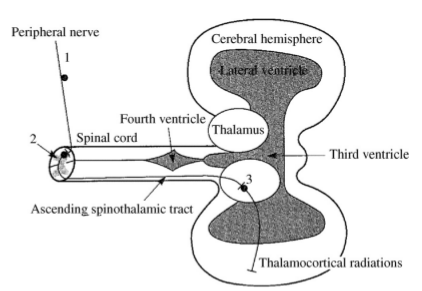
\includegraphics[width=0.7\linewidth]{figura_2.png} 
%\caption{A simplified diagram of the CNS showing a typical general sense
%pathway from the periphery (neuron 1) to the brain (neuron 3). Note that the
%axon of the secondary neuron (neuron 2) in the pathway decussates (crosses) to
%the opposite side of the cord. Descending (motor) pathways are also crossed
%(see text).}
%\end{figure}
%
%either the spinal cord [e.g., the dorsal horn or the brain stem (Figure 4.25)].
%Note from Figure 4.25 that the axon of the secondary neuron crosses (decus-
%sates) to the other side of the cord and joins a nerve fiber tract bound for the
%thalamus. The tertiary neuron in the pathway is located in a thalamic nucleus,
%and its axon travels in the thalamocortical radiations to the postcentral gyrus,
%which is located just posterior to the central sulcus [Figure 4.24 (inset)]. Thus,
%the postcentral gyrus is the cortical projection area for the general senses.
%Neural pathways for the special senses, particularly audition and vision,
%follow the same general ground plan; however, there are notable deviations
%from the scheme depicted in Figure 4.25. Usually, more than three neurons are
%involved in the pathway and not all of the ‘‘secondary neurons’’ decussate.
%Most of the neurons cross to the opposite (contralateral) side of the body,
%however a significant number ascend to the thalamus on the same (ipsilateral)
%side of the body. The auditory and visual pathways have their own special
%thalamic relay centers—the medial and lateral geniculate bodies, respectively,
%as well as their own cortical projection areas (Figure 4.24).
%Likewise, within the CNS there are descending (motor) nerve tracts that
%originate in various brain structures such as the cerebrum and cerebellum
%(Figure 4.24) and terminate ultimately on motor neurons in the ventral horn of
%the spinal cord (Figure 4.10). These motoneurons, in turn, control the con-
%tractile activity of the skeletal musculature. For example, the corticospinal
%tract is a bundle of axons from the primary motor cortex [precentral gyrus,
%Figure 4.24 (inset)], which projects directly to motor neurons in the spinal cord.
%Since the ascending general sensory pathways are crossed, the descending
%corticospinal tracts each cross to the opposite side of the body prior to making
%synaptic contact with the spinal motor neurons.
%Thus, two-way communication links exist between the brain and spinal
%cord that allow higher centers in the brain to control or modify the behavior of
%the elemental spinal reflex arc at a given spinal level. By means of these links,
%the brain is not only informed of a peripheral event but can also modify the
%response of the spinal reflex to that environmental stimulus. Information is
%transmitted to the brain by means of a frequency-modulated train of nerve
%impulses that, upon reaching specific areas of the brain, stimulates the activity
%of resident neurons. Similarly, the decision to implement a motor action in
%response to the initial stimulus is manifested in the electrical activity of cortical
%neurons in specific areas of the brain [e.g., precentral gyrus (primary motor
%cortex); premotor cortex in frontal lobe]. The pattern of activity is specific to
%the type of motor action to be taken.
%Electrical activity in either ascending or descending nerve fiber tracts may
%be represented to a first approximation by an action current dipole oriented in
%the direction of propagation (bioelectric source model). One should be aware
%that the properties (e.g., size, bulk conductivity) of the volume-conductor
%medium can change along the length of a particular fiber tract between the
%spinal cord and the cortex, and the volume-conductor model adopted should
%be based on the particular measurement considered. The volume-conductor-
%field potential solutions can be used to both fit and interpret body surface
%
%potential measurements obtained clinically. Recording field potentials non-
%invasively from the relatively small volume of active nerve trunks, invariably
%requires the use of cumulative signal averaging techniques. In Figure 4.8, the
%median nerve was stimulated and compound action potentials were recorded
%from the subject’s forearm. Although not shown in this figure, sensory fibers in
%the median nerve thus activated, initiate activity in the general sense pathways
%to the brain. Averaged field potential recordings can be taken at a variety of
%points along the ascending pathways [e.g., from spinal cord and brain stem
%tracts taking note of the crossed nature of the pathway, and finally at the cortex
%itself (postcentral gyrus)]. The field potentials associated with long nerve tracts
%depends to a large extent on (a) whether the tract is straight or bent and (b) the
%resistance (geometry and specific conductivity) of the surrounding volume-
%conductor media.
%This important subject is discussed later; however, for the present, these
%different types of averaged field potentials are called collectively somato-
%sensory evoked potentials. The subject of nerve tracts has been discussed
%previously; however, the activity of both nuclei in the ascending pathway
%and clusters of cells in the cortex, depends not only on the ensemble of neurons
%there, but also on the geometry of the ensemble and the different types of
%synaptic connections involved.
%Averaged sensory evoked potentials in response to brief auditory ‘‘clicks’’
%or flashes of light are also routinely recorded as the auditory evoked response
%(AER) and the visual evoked response (VER), respectively (Jacobson, 1994;
%Heckenlively and Arden, 1991). Using an electromagnetic stimulating device
%held over the primary motor cortex (just anterior to the central sulcus), it is
%also possible to induce currents that activate the corticospinal tract, making
%possible the recording of averaged field potentials from the descending motor
%pathways (York, 1987; Geddes, 1987; Esselle and Stuchly, 1992). The same
%volume-conductor principles are applicable to the analysis of these different
%types of evoked potential recordings. The cerebrum is a paired structure, with
%right and left cerebral hemispheres, each relating to the opposite side of the
%body. That is, voluntary movements of the right hand are ‘‘willed’’ by the left
%cerebral hemisphere. The surface layer of the hemisphere is called the cortex;
%it receives sensory information from skin, eyes, ears, and other receptors
%located generally on the opposite side of the body. This information is
%compared with previous experience and produces movements in response
%to these stimuli.
%Each hemisphere consists of several layers. The outer layer is a dense
%collection of nerve cells that appear gray in color when examined in a fresh
%state. It is consequently called gray matter. This outer layer, roughly 1 cm thick,
%is called the cerebral cortex. It has a highly convoluted surface consisting of gyri
%(ridges) and sulci (valleys), the deeper sulci being termed fissures. The deeper
%layers of the hemisphere (beneath the cortex) consist of myelinated axons (or
%white matter) and collections of cell bodies termed nuclei. Some of the
%integrative functions of the cerebrum can be localized within certain regions
%of the cortex; others are more diffusely distributed.
%
%A major dividing landmark of the cerebral cortex is the lateral fissure
%(Figure 4.24), which runs on the lateral (side) surface of the brain from the
%open end in front, posteriorly and dorsally (backward and upward). The lateral
%fissure defines a side lobe of cortex inferior to (below) it that is called the
%temporal lobe [Figure 4.24 (inset)]. The superior (upper) part of this lobe
%contains the primary auditory cortex, which is the part of the cortex that
%receives auditory impulses via neural pathways leading from the auditory
%receptors in the inner ear.
%The visual system is another example of the projection of the senses onto
%the cerebral cortex. The occipital lobe at the back of the head is the primary
%visual cortex. Light flashed into the eye evokes large electrical potentials from
%electrodes placed over this area of the cortex.
%Another major landmark of the cerebral cortex is the central sulcus
%[Figure 4.24 (inset)]. However, it is not so prominent and unvarying an
%anatomical landmark as the lateral fissure. The central sulcus runs from
%the medial surface (surface along the midline of the brain) over the convexity
%of the hemisphere to the lateral fissure. It also represents the posterior border
%of the frontal lobe. The gyrus lying just anterior (forward) to the central sulcus
%is the precentral gyrus, which functions as the primary motor cortex. From this
%gyrus, nerve signals run down through the brainstem to the spinal cord for
%control of skeletal muscles via neural control of motoneurons in the ventral
%horn of the spinal cord (Figure 4.10). Lesions (destruction) of part of the
%precentral gyrus cause partial paralysis on the opposite side of the body.
%Immediately posterior to the central sulcus [Fig. 24 (inset)] is the primary
%somatosensory cortex, the postcentral gyrus. This region receives impulses from
%all the general sense receptors from the skin (such as pressure, touch, and pain
%receptors). Each little area along this gyrus is related to a particular part of the
%body (for example, the legs on the medial end, the hand in the center, and the
%face on the end next to the lateral fissure). If a recording electrode is placed
%appropriately during a neurosurgical procedure, a cortical response can be
%evoked by tactile stimuli delivered to the contralateral (opposite) hand. Like-
%wise, if a stimulus is applied through the same electrode, the subject reports a
%tingling sensation in the contralateral hand. Higher-order sensory discrimina-
%tion, such as the ability to recognize a number drawn on the palm of the hand,
%is organized solely in the parietal lobe of which the postcentral gyrus is a part.
%Destruction of the parietal lobe results in a loss of this discriminative ability.
%For example, a subject may still know that he or she is being touched but
%cannot tell where or what is being drawn on the palm of the hand. The parietal
%lobe is also responsible for a person’s awareness of the general position of the
%body and its limbs in space.
%
%\subsection{ULTRASTRUCTURE OF THE CEREBRAL CORTEX}
%
%The functional part of the cerebrum is the cerebral cortex (bark, outer
%covering), a relatively thin layer of gray matter (1.5 to 4.0 mm in thickness)
%covering the outer surface of the cerebrum, including its intricate convolutions.
%
%Because it is the most recent phylogenetic acquisition of the brain, the cerebral
%cortex has undergone a relatively greater development than other parts of the
%brain. The greatest advance in relative growth has been the neocortex, which is
%present on the superior and lateral aspects of the cerebral hemispheres. The
%distinctly different type of cortex located on the medial surface and base of the
%brain is known as the paleocortex. We shall use the term cortex in this chapter
%to refer specifically to the neocortex.
%Cortical architectures in vertebrates share several common features:
%(1) stratified layers containing cell bodies and fiber bundles; (2) an outermost
%layer that lacks neurons (layer I); (3) at least one inner layer containing
%neurons that give rise to large dendrites, which rise vertically to layer I and
%travel in that layer forming multiple branches (arborization). The human
%cortex is generally arranged in six such cortical layers. The neurons are of two
%main types: pyramidal and nonpyramidal (many subtypes have been identi-
%fied). There are also a large number of horizontally oriented layers of nerve
%fibers that extend between adjacent regions of the cortex, as well as vertically
%oriented bundles that extend from the cortex to more distant regions of the
%cortex or downward to the brainstem and spinal cord.
%Figure 4.26 shows a schematic drawing of a typical cortical pyramidal
%cell. The bodies of this type of cell are commonly triangular in shape, with
%the base down and the apex directed toward the cortical surface. (Pyramidal
%
%\begin{figure}
%\centering
%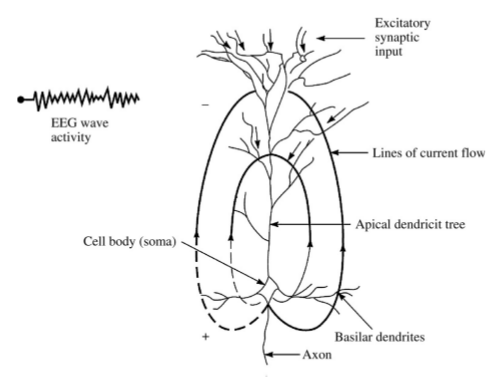
\includegraphics[width=0.7\linewidth]{figura_3.png} 
%\caption{Electrogenesis of cortical field potentials for a net excitatory
%input to the apical dendritic tree of a typical pyramidal cell. For the case of a
%net inhibitory input, polarity is reversed and the apical region becomes a
%source (nose). Current flow to and from active fluctuating synaptic knobs on the
%dendrites produces wavelike activity. (See text.)}
%\end{figure}
%
%cell bodies vary greatly in size, from axial dimensions of 15 x 10 mm up to
%120 x 90 mm or more for the giant pyramids of the motor cortex, which are
%called Betz cells after their discoverer.) These cells usually consist of the
%following parts: (1) a long apical dendrite (up to 2 mm in length) that ascends
%from the apex of the cell body through the overlaying cellular layers, and
%which frequently reaches and branches terminally within the outermost
%layer of the cortex; (2) dense dendritic arborization occurring at the base
%of the pyramid-shaped cell (largely horizontally—basilar dendrites); and (3)
%a single pyramidal cell axon which can emerge from the inner surface of the
%cortex as projection fibers to other areas of the cortex, or to other structures
%(e.g., the thalamus, cerebellum, or spinal cord). Frequently these axons send
%recurrent collateral (feedback) branches back on the cellular regions from
%which they sprang. Axons of some pyramidal cells turn back toward the
%cortical surface (never leaving the gray matter) to end via their many
%branches on the dendrites of other cells.
%Nonpyramidal cells of the neocortex differ remarkably from pyramidal
%cells. Their cell bodies are small, and dendrites spring from them in all
%directions to ramify in the immediate vicinity of the cell. The axon may arise
%from a large dendrite; it commonly divides repeatedly to terminate on the cell
%bodies and dendrites of immediately adjacent cells. The axons of other non-
%pyramidal cells may turn upward toward the cortical surface, or they may leave
%the motor cortex (though this is not common).
%For a detailed exposition of the various cells, layers, cellular interconnec-
%tions, inputs, and outputs of the neocortex, see Kandel et al. (1991).

%%%%%%%%%%%%%%%%%%%%%%%%%%%%%%%%%%%%%%%%%%%%%%%%%%%%%%%%%%%%%%%%%%%%%%%%%%%%%%%%%%%%%%%%%%%%%%%%%%%

\subsection{BIOELECTRIC POTENTIALS FROM THE BRAIN}

Unipolar recordings of the cortical surface potential relative to that of a
remote reference potential may be viewed as a measurement of the integrated
field potential at a boundary of a large volume conductor that contains an array
of action current sources. Under normal conditions, action potentials con-
ducted by axons in the cortical medium contribute very little to the integrated
surface potential, since there are many axons in the cortex which run in many
directions relative to the surface and which fire asynchronously. Consequently,
their net spatial and temporal influence on the field potential at the surface is
negligible. An exception occurs, of course, in the case of a response evoked by
the simultaneous (synchronous) stimulation of a cortical input (e.g., direct
electrical stimulation of thalamic nuclei or their afferent pathways, which
project directly to the cortex via thalamocortical axons—the cortical input).
These synchronous responses are called evoked potentials, and they are of
relatively large amplitude. Synchronicity of the underlying fiber and cortical
neuron activity is a major factor influencing surface potential magnitude.
Unipolar field potentials recorded within the cortical layers have shown
that the cortical surface potential is largely due to the net effect of local
postsynaptic potentials of cortical cells (Figure 4.26). These may be of either
sign (excitatory or inhibitory) and may occur directly underneath the electrode

or at some distance from it. A potential change recorded at the surface is a
measure of the net potential (current resistance iR) drop between the surface
site and the distant reference electrode. It is obvious, however, that if all the
cell bodies and dendrites of cortical cells were randomly arranged in the
cortical medium, the net influence of synaptic currents would be zero. This
would result in a ‘‘closed field’’ situation that produces relatively small far-field
potentials (Lorente de No, 1947). Thus, any electrical change recorded at the
surface must be due to the orderly and symmetric arrangement of some class of
cells within the cortex.
Pyramidal cells of the cerebral cortex are oriented vertically, with their
long apical dendrites running parallel to one another. Potential changes in one
part of the cell relative to another part create ‘‘open’’ potential fields in which
current may flow and potential differences can be measured at the cortical
surface. Figure 4.26 illustrates this concept in diagrammatic fashion. Synaptic
inputs to the apical dendritic tree cause depolarization of the dendritic
membrane. As a result, subthreshold current flows in a closed path through
the cytoplasmic core of the dendrites and cell body of the pyramidal cell,
returning ultimately to the surface synaptic sites via the extracellular bathing
medium. From the indicated direction of the lines of current flow, the
extracellular medium about the soma behaves as a source (nose), while the
upper part of the apical dendritic tree behaves as a sink ().
The influence of a particular dendritic postsynaptic potential (PSP) on the
cortical surface recording depends on its sign [excitatory () or inhibitory ()]
and on its location relative to the measurement site. The effect of each PSP
may be regarded as creating a radially oriented current dipole. Therefore,
continuing synaptic input creates a series of potential dipoles and resulting
current flows that are staggered but overlapped in space and time. Surface
potentials of any form can be generated by one population of presynaptic fibers
and the cells on which they terminate, depending on the proportion that are
inhibitory or excitatory, the level of the postsynaptic cells in the cortex, and so
forth.
Nonpyramidal cells in the neocortex, on the other hand, are unlikely to
contribute substantially to surface records. Their spatially restricted dendritic
trees are radially arranged around their cell bodies such that charge differences
between the dendrites and the cell body produce fields of current flow that sum
to zero when viewed from a relatively great distance on the cortical surface
(closed-field situation).
Thus, to summarize, the apical dendrites of pyramidal cells constitute a
meshwork of similarly oriented, densely packed units in the outer layers of the
cortex. As multiple synaptic endings on the dendritic tree of each cell become
active, current can flow in either direction between the dendritic process
depending on whether the synapses are excitatory or inhibitory. The
source–sink relationship between dendrite and cell is that of a constantly
shifting current dipole, where variations in dipole orientation and strength
produce wavelike fluctuations in the surface field potential (Figure 4.26).
When the sum of dendritic activity is negative relative to the cell, the cell

is depolarized and quite excitable. When it is positive, the cell is hyper-
polarized and less excitable.

%%%%%%%%%%%%%%%%%%%%%%%%%%%%%%%%%%%%%%%%%%%%%%%%%%%%%%%%%%%%%%%%%%%%%%%%%%%%%%%%%%%%%%%%%%%%%%%%%%%

\subsection{RESTING RHYTHMS OF THE BRAIN}

Electric recordings from the exposed surface of the brain or from the outer
surface of the head demonstrate continuous oscillating electric activity within
the brain. Both the intensity and the patterns of this electric activity are
determined to a great extent by the overall excitation of the brain resulting
from functions in the brainstem reticular activating system (RAS). The
undulations in the recorded electric potentials (Figure 4.27) are called brain
waves, and the entire record is called an electroencephalogram (EEG).

\begin{figure}
\centering
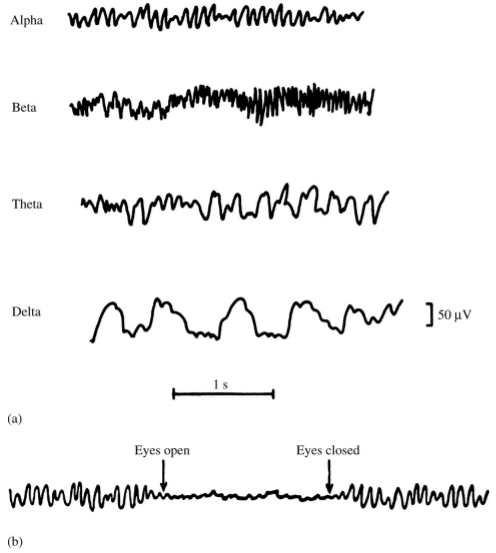
\includegraphics[width=0.7\linewidth]{figura_4.png} 
\caption{(a) Different types of normal EEG waves. (b) Replacement of
alpha rhythm by an asynchronous discharge when patient opens eyes.
(c) Representative abnormal EEG waveforms in different types of epilepsy.
(From A. C. Guyton, Structure and Function of the Nervous System, 2nd ed.,
Philadelphia: W.B. Saunders, 1972; used with permission.)}
\end{figure}

\begin{figure}
\centering
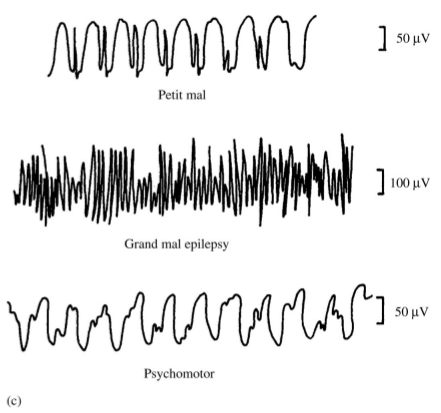
\includegraphics[width=0.7\linewidth]{figura_5.png} 
\caption{(Continuation)}
\end{figure}

relative to an indifferent electrode such as the earlobe) may be as large as 10 mV,
whereas those recorded from the scalp have a smaller amplitude of approximately
100 mV. The frequencies of these brain waves range from 0.5 to 100 Hz, and their
character is highly dependent on the degree of activity of the cerebral cortex. For
example, the waves change markedly between states of wakefulness and sleep.
Much of the time, the brain waves are irregular, and no general pattern can be
observed. Yet at other times, distinct patterns do occur. Some of these are
characteristic of specific abnormalities of the brain, such as epilepsy (discussed
later). Others occur in normal persons and may be classified as belonging to one of
four wave groups (alpha, beta, theta, and delta), which are shown in Figure 4.27(a).
Alpha waves are rhythmic waves occurring at a frequency between 8 and
13 Hz. They are found in EEGs of almost all normal persons when they are
awake in a quiet, resting state of cerebration. These waves occur most intensely
in the occipital region but can also be recorded, at times, from the parietal and
frontal regions of the scalp. Their voltage is approximately 20 to 200 mV. When
the subject is asleep, the alpha waves disappear completely. When the awake
subject’s attention is directed to some specific type of mental activity, the alpha
waves are replaced by asynchronous waves of higher frequency but lower
amplitude. Figure 4.27(b) demonstrates the effect on the alpha waves of simply
opening the eyes in bright light and then closing them again. Note that the
visual sensations cause immediate cessation of the alpha waves; these are
replaced by low-voltage, asynchronous waves.

Beta waves normally occur in the frequency range of 14 to 30 Hz, and
sometimes—particularly during intense mental activity—as high as 50 Hz.
These are most frequently recorded from the parietal and frontal regions of the
scalp. They can be divided into two major types: beta I and beta II. The beta I
waves have a frequency about twice that of the alpha waves. They are affected
by mental activity in much the same way as the alpha waves (they disappear
and in their place appears an asynchronous, low-voltage wave). The beta II
waves, on the other hand, appear during intense activation of the central
nervous system and during tension. Thus one type of beta activity is elicited by
mental activity, whereas the other is inhibited by it.
Theta waves have frequencies between 4 and 7 Hz. These occur mainly in
the parietal and temporal regions in children, but they also occur during
emotional stress in some adults, particularly during periods of disappointment
and frustration. For example, they can often be brought about in the EEG of a
frustrated person by allowing the person to enjoy some pleasant experience
and then suddenly removing the element of pleasure. This causes approxi-
mately 20 s of theta waves.
Delta waves include all the waves in the EEG below 3.5 Hz. Sometimes
these waves occur only once every 2 or 3 s. They occur in deep sleep, in infancy,
and in serious organic brain disease. They can also be recorded from the brains
of experimental animals that have had subcortical transections producing a
functional separation of the cerebral cortex from the reticular activating
system. Delta waves can thus occur solely within the cortex, independent of
activities in lower regions of the brain.
A single cortical cell can give rise only to small extracellular current, so large
numbers of neurons must be synchronously active to give rise to the potentials
recorded from the cerebral surface. The individual waves of the EEG are of long
duration (for example, 30 to 500 ms), and one might well ask how they are
produced. They can be long-lasting depolarizations of the cell membranes (for
example, of the apical dendrites of pyramidal cells) or a summation of a number
of shorter responses. In any event, a sufficiently large number of neurons must
discharge together to give rise to these cortical potentials. The term synchroni-
zation is used to describe the underlying process that acts to bring a group of
neurons into unified action. Synaptic interconnections are generally thought to
bring about synchronization, although extracellular field interaction between

cells has been proposed as a possible mechanism. Rhythmically firing neurons are
very sensitive to voltage gradients in their surrounding medium.
Besides the synchronization required for each wave of resting EEG, the series
of repeated waves suggests a rhythmic and a trigger or pacemaker process that
initiates such rhythmic action. By means of knife cuts below the intact connective-
tissue covering (meningeal layer or pia matter) of the brain, one may prepare
chronic islands of cortex—with all neuronal connections cut, but with the blood
supply via surface vessels intact. Only a low level of EEG activity remains in such
islands. Though the isolated islands of cortex may not show spontaneous EEG
activity, they still have the ability to respond rhythmically, which may be readily
demonstrated by the rhythmic responses that are elicited by applying a single
electrical stimulus. The inference is that various regions of the cortex, though
capable of exhibiting rhythmic activity, require trigger inputs to excite rhythmic-
ity. The RAS, mentioned earlier, appears to provide this pacemaker function.

%%%%%%%%%%%%%%%%%%%%%%%%%%%%%%%%%%%%%%%%%%%%%%%%%%%%%%%%%%%%%%%%%%%%%%%%%%%%%%%%%%%%%%%%%%%%%%%%%%%

\subsection{THE CLINICAL EEG}

The system most often used to place electrodes for monitoring the clinical
EEG is the International Federation 10–20 system shown in Figure 4.28. This
system uses certain anatomical landmarks to standardize placement of EEG
electrodes. The representation of the EEG channels is referred to as a
montage. In the bipolar montage, each channel measures the difference
between two adjacent electrodes. In the referential montage, each channel

\begin{figure}
\centering
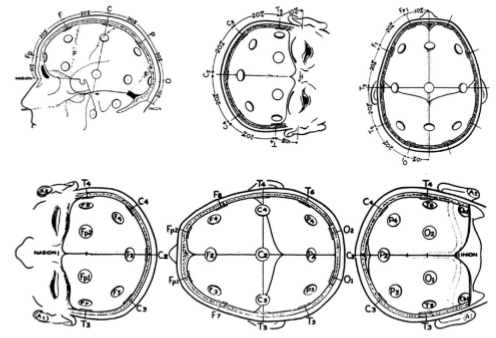
\includegraphics[width=0.7\linewidth]{figura_6.png} 
\caption{The 10–20 electrode system This system is recommended by the
International Federation of EEG Societies. [From H. H. Jasper, ‘‘The ten–
twenty electrode system of the International Federation in Electroencepha-
lography and Clinical Neurophysiology.’’ EEG Journal, 1958, 10 (Appendix),
371–375.]}
\end{figure}

measures the diffference between one electrode and a reference electrode,
such as on the ear. In the average reference montage, each channel measures
the difference between one electrode and the average of all other electrodes.
In the Laplacian montage, each channel measures the difference between one
electrode and a weighted average of the surrounding electrodes. The differ-
ential amplifier requires a separate ground electrode plus differential inputs to
the electrode connections. The advantage of using a differential recording
between closely spaced electrodes (between successive pairs in the standard
system, for example) is cancellation of far-field activity common to both
electrodes; one thereby obtains sharp localization of the response. Although
the same electric events are recorded in each of the ways, they appear in a
different format in each case. The potential changes that occur are amplified by
high-gain, differential, capacitively coupled amplifiers. The output signals are
recorded and displayed.
In the routine recording of clinical EEGs, the input electrodes are a
problem. They must be small, they must be easily affixed to the scalp with
minimal disturbance of the hair, they must cause no discomfort, and they must
remain in place for extended periods of time. Technicians prepare the surface
of the scalp, degrease the recording area by cleaning it with alcohol, apply a
conducting paste, and glue nonpolarizable Ag/AgCl electrodes to the scalp
with a glue (collodion) and hold them in place with rubber straps, or use a
rubber cap that contains all electrodes.
The EEG is usually recorded with the subject awake but resting recumbent
on a bed with eyes closed. With the patient relaxed in such a manner, artifacts
from electrode-lead movement are significantly reduced, as are contaminating
signals from the scalp. Muscle activity from the face, neck, ears, and so on is
perhaps the most subtle contaminant of EEG records in the recording of both
spontaneous ongoing activity in the brain and activity evoked by a sensory
stimulus (evoked response). For example, the frequency spectrum of the field
produced by mildly contracted facial muscles contains frequency components
well within the nominal EEG range (0.5 to 100 Hz). After technicians have
achieved resting, quiescent conditions in the normal adult subject, the subject’s
scalp recordings show a dominant alpha rhythm in the parietal-occipital areas,
whereas in the frontal areas, there is a low-amplitude, higher-frequency beta
rhythm in addition to the alpha rhythm. In the normal subject there is
symmetry between the recordings of the right and left hemispheres. There
can be a wide range of EEG measurement artifacts.
In general there is a relationship between the degree of cerebral activity
and the average frequency of the EEG rhythm: The frequency increases
progressively with higher and higher degrees of activity. For example, delta
waves are frequently found in stupor, surgical anesthesia, and sleep; theta
waves in infants; alpha waves during relaxed states; and beta waves during
intense mental activity. However, during periods of mental activity, the waves
usually become asynchronous rather than synchronous, so that the magnitude
of the summed surface potential recording decreases despite increased cortical
activity.

%%%%%%%%%%%%%%%%%%%%%%%%%%%%%%%%%%%%%%%%%%%%%%%%%%%%%%%%%%%%%%%%%%%%%%%%%%%%%%%%%%%%%%%%%%%%%%%%%%%

\subsection{SLEEP PATTERNS}

When an individual in a relaxed, inattentive state becomes drowsy and falls
asleep, the alpha rhythm is replaced by slower, larger waves (Figure 4.29). In
deep sleep, very large, somewhat irregular delta waves are observed. Inter-
spersed with these waves—during moderately deep sleep—are bursts of alpha-
like activity called sleep spindles. The alpha rhythm and the patterns of the
drowsy and sleeping subject are synchronized, in contrast with the low-voltage
desynchronized, irregular activity seen in the subject who is in an alert state.
The high-amplitude, slow waves seen in the EEG of a subject who is asleep
are sometimes replaced by rapid, low-voltage irregular activity resembling that
obtained in alert subjects. However, the sleep of a subject with this irregular
pattern is not interrupted; in fact, the threshold for arousal by sensory stimuli is
elevated. This condition has therefore come to be called paradoxical sleep.
During paradoxical sleep, the subject exhibits rapid, roving eye movements.
For this reason, it is also called rapid-eye-movement sleep, or REM sleep.
Conversely, spindle or synchronized sleep is frequently called nonrapid-eye-
movement (NREM), or slow-wave sleep. Human subjects aroused at a time
when their EEG exhibits a paradoxical (REM) sleep pattern generally report

\begin{figure}
\centering
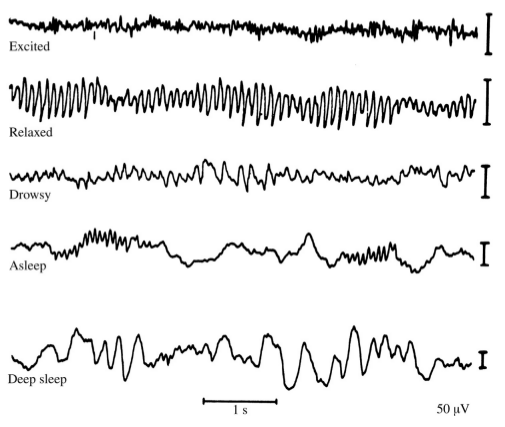
\includegraphics[width=0.7\linewidth]{figura_7.png} 
\caption{The electroencephalographic changes that occur as a human subject
goes to sleep The calibration marks on the right represent 50 mV. (From H.
H. Jasper, ‘‘Electrocephalography.’’ In Epilepsy and Cerebral Localization, W.
G. Penfield and T. C. Erickson (eds.). Springfield, IL: Charles C. Thomas,
1941.)}
\end{figure}

that they were dreaming, whereas individuals wakened from spindle sleep do
not. This observation and other evidence indicate that REM sleep and
dreaming are closely associated. It is interesting that during REM sleep, there
is a marked reduction in muscle tone, despite the rapid eye movements.

%%%%%%%%%%%%%%%%%%%%%%%%%%%%%%%%%%%%%%%%%%%%%%%%%%%%%%%%%%%%%%%%%%%%%%%%%%%%%%%%%%%%%%%%%%%%%%%%%%%

\subsection{THE VOLUME-CONDUCTOR PROBLEM IN ELECTROENCEPHALOCRAPHY}

Geometrically speaking, the brain approximates a sphere surrounded by
concentric shells that differ in impedance and comprise the meninges (connec-
tive tissue coverings of the brain), cerebral spinal fluid, skull, and scalp. This
model is inaccurate to the extent that the brain is not really a true sphere, and
its coverings are irregular in shape and thickness. Such irregularities are
insignificant for the upper half of the brain, but complications are introduced
by the marked departure of the lower parts of the brain from a spherical shape,
as well as by variations in impedance produced by the openings (to the spinal
column) through the base of the shell. Various cerebral structures differ
somewhat in specific resistivity. Resistivity also varies in relation to the
predominant direction of the fibers within the white matter. Thus the brain
is neither a homogeneous nor an isotropic conducting medium.
In practice, neurological generators do not correspond precisely to simple,
one-dimensional dipoles. Any source of activity large enough to manifest itself
in the EEG constitutes at least a small area of the cortex containing synchro-
nously active neurons. This source may be regarded as a three-dimensional
sheet polarized across its thickness. If it is small enough, it may still be
conveniently represented as an equivalent dipole per unit volume. A larger
area of the cortex may be curved, or even convoluted, and the equivalent
dipole then becomes a complex vector sum of the whole. When there are many
widely scattered active-current generators, an infinite number of combinations
may give rise to the same pattern of surface potentials.
Determining the equivalent dipole of cerebral activity is therefore of
practical value only when EEG sources are highly ‘‘focal.’’ Fortunately, this
condition occurs frequently in the brain’s response to sensory stimulation, as
well as in pathological conditions. For example, Nunez (1981) considers in
some depth the subject of the calculation of field potentials from equivalent
current sources in inhomogeneous media. Particularly in Chapter of his book,
Nunez provides an introduction to the equivalent source models that have
been used in the field of theoretical electroencephalography to interpret scalp
potentials. Examples of these models include the simple dipole at the center of
a spherical conducting medium, the radially oriented dipole not at the center of
a sphere (the radially oriented eccentric dipole), the freely oriented eccentric
dipole in a sphere, the dipole in a three-concentric spherical shell model, and a
dipole current source below a multilayered planar conducting medium.
Considerable interest has arisen in determining the location of intra-
cerebral sources of the potentials that are measured on the scalp. In general,
nonuniqueness of this inverse problem is well known in that different

configurations of sources can lead to the same surface distribution. The usual
approach taken to obtaining an approximate solution to the inverse problem is
as follows:
1.
2.
3.
4.
Assume a model (such as the eccentrically located dipole in a uniform,
homogeneous spherical conducting medium. Assume that the electric
field is quasistatic).
After obtaining a solution to the associated boundary-value problem (the
forward problem), produce model-generated potential values at measure-
ment points on the cortical surface.
Compare these theoretical potential values with particular discrete-time
values of EEG waveforms measured at the same surface sites, and form a
general least-squares reconstruction error function wherein the error is
defined as the difference between predicted and measured potential at
several selected cortical measurement sites.
Iteratively adjust the EEG dipolar source parameters at each discrete-
time instant to obtain the best fit to sampled EEG waveforms in a least-
squares sense. The optimal dipole location is assumed to be the dipole
location obtained when the reconstruction error function is so minimized.
The influence of anisotropy on various EEG phenomena has been studied
using models [Henderson et al. (1975); Cuffin (1991); Haueisen et al. (2002)].
These investigations, together with various in vivo studies, substantially agree
that the presence of tissue anisotropy tends to attenuate and smear the pattern
of scalp-recorded EEGs. However, this type of amplitude-related degradation
apparently does not affect the model’s ability to predict the locus of the EEG
equivalent-dipole generator (although the dipole moment might be under-
estimated). This is important in the sense that one of the major objectives of
electroencephalography is determination of source location—for localized or
focal activity—because in case of evoked cortical potentials and deep-brain
pathologies, this concept of an equivalent-dipole generator is of clinical value.

\subsection{THE ABNORMAL EEG}

One of the more important clinical uses of the EEG is in the diagnosis of
different types of epilepsy and in the location of the focus in the brain causing
the epilepsy. Epilepsy is characterized by uncontrolled excessive activity by
either a part or all of the CNS. A person predisposed to epilepsy has attacks
when the basal level of excitability of all or part of the nervous system rises
above a certain critical threshold. However, as long as the degree of excitability
is held below this threshold, no attack occurs.
There are two basic types of epilepsy, generalized epilepsy and partial
epilepsy. Generalized epilepsy involves the entire brain at once, whereas
partial epilepsy involves a portion of the brain—sometimes only a minute
focal spot and at other times a fair amount of the brain. Generalized epilepsy is
further divided into grand mal and petit mal epilepsy.

Grand mal epilepsy is characterized by extreme discharges of neurons
originating in the brainstem portion of the RAS. These discharges then spread
throughout the cortex, to the deeper parts of the brain, and even to the spinal
cord to cause generalized tonic convulsions of the entire body. They are
followed near the end of the attack by alternating muscular contractions, called
clonic convulsions. The grand mal seizure lasts from a few seconds to as long as
3 to 4 min and is characterized by postseizure depression of the entire nervous
system. The subject may remain in a stupor for 1 min to as long as a day or more
after the attack is over.
The middle recording in Figure 4.27(c) shows a typical EEG during a
grand mal attack. This response can be recorded from almost any region of the
cortex. The recorded potential is of a high magnitude, and the response is
synchronous, with the same periodicity as normal alpha waves. The same type
of discharge occurs on both sides of the brain at the same time, indicating that
the origin of the abnormality is in the lower centers of the brain that control the
activity of the cerebral cortex, not in the cortex itself. Electrical recordings
from the thalamus and reticular formation of experimental animals during an
induced grand mal attack indicate typical high-voltage synchronous activity in
these areas, similar to that recorded from the cerebral cortex. Experiments on
animals have further shown that a grand mal attack is caused by intrinsic
hyperexcitability of the neurons that make up the RAS structures or by some
abnormality of the local neural pathways of this system.
Petit mal epilepsy is closely allied to grand mal epilepsy. It occurs in two
forms, the myoclonic form and the absence form. In the myoclonic form, a
burst of neuronal discharges, lasting a fraction of a second, occurs throughout
the nervous system. These discharges are similar to those that occur at the
beginning of a grand mal attack. The person exhibits a single violent muscular
jerk involving arms or head. The entire process stops immediately, however,
and the attack is over before the subject loses consciousness or stops what he or
she is doing. This type of attack often becomes progressively more severe until
the subject experiences a grand mal attack. Thus the myoclonic form of petit
mal is similar to a grand mal attack, except that some form of inhibitory
influence promptly stops it.
The absence type of petit mal epilepsy is characterized by 5 to 20 s of
unconsciousness, during which the subject has several twitchlike contractions
of the muscles, usually in the head region. There is a pronounced blinking of
the eyes, followed by a return to consciousness and continuation of previous
activities. This type of epilepsy is also closely allied to grand mal epilepsy. In
rare instances, it can initiate a grand mal attack.
Figure 4.27(c) shows a typical spike-and-dome pattern that is recorded
during the absence type of petit mal epilepsy. The spike portion of the record is
almost identical to the spikes occurring in grand mal epilepsy, but the dome
portion is distinctly different. The spike-and-dome pattern can be recorded
over the entire cortex, illustrating again that the seizure originates in the RAS.
Partial epilepsy can involve almost any part of the brain, either localized
regions of the cerebral cortex or deeper structures of both the cerebrum and

brainstem. Partial epilepsy almost always results from some organic lesion of
the brain, such as a scar that pulls on the neuronal tissue, a tumor that
compresses an area of the brain, or a destroyed region of the brain tissue.
Lesions such as these can cause local neurons to fire very rapid discharges.
When the rate exceeds approximately 1000/s, synchronous waves begin
spreading over adjacent cortical regions. These waves presumably result
from the activity of localized reverberating neuronal circuits that gradually
recruit adjacent areas of the cortex into the ‘‘discharge,’’ or firing, zone. The
process spreads to adjacent areas at rates as slow as a few millimeters per
minute to as fast as several centimeters per minute. When such a wave of
excitation spreads over the motor cortex, it causes a progressive ‘‘march’’ of
muscular contractions throughout the opposite side of the body, beginning
perhaps in the leg region and marching progressively upward to the head
region, or at other times marching in the opposite direction. This is called
Jacksonian epilepsy or Jacksonian march.
Another type of partial epilepsy is the so-called psychomotor seizure,
which may cause (1) a short period of amnesia, (2) an attack of abnormal rage,
(3) sudden anxiety or fear, (4) a moment of incoherent speech or mumbling, or
(5) a motor act of rubbing the face with the hand, attacking someone, and so
forth. Sometimes the person does not remember his or her activities during the
attack; at other times the person is completely aware of, but unable to control,
his or her behavior. The bottom tracing of Figure 4.27(c) represents a typical
EEG during a psychomotor seizure showing a low-frequency rectangular-wave
response with a frequency between 2 and 4 Hz with superimposed 14 Hz waves.
The EEG frequently can be used to locate tumors and also abnormal
spiking waves originating in diseased brain tissue that might predispose to
epileptic attacks. Once such a focal point is found, surgical excision of the focus
often prevents future epileptic seizures.
The EEG is also used to monitor the depth of anesthesia.
The EEG is also used as a brain–computer interface to enable disabled
persons to communicate with a computer.

%%%%%%%%%%%%%%%%%%%%%%%%%%%%%%%%%%%%%%%%%%%%%%%%%%%%%%%%%%%%%%%%%%%%%%%%%%%%%%%%%%%%%%%%%%%%%%%%%%%
%%%%%%%%%%%%%%%%%%%%%%%%%%%%%%%%%%%%%%%%%%%%%%%%%%%%%%%%%%%%%%%%%%%%%%%%%%%%%%%%%%%%%%%%%%%%%%%%%%%